	\begin{figure}[h]
	\centering
		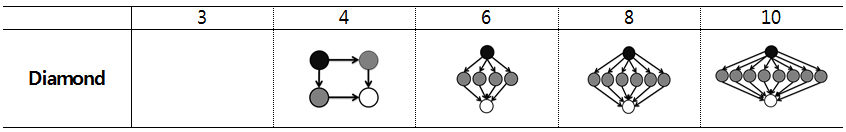
\includegraphics[height=50pt]{Topologies_Diamond}
		\caption{Bayesian Network Topologies : Diamond}
	\end{figure}	

	% Diamond는 윗 부분은 한 개의 node가 여러 개의 자식 node를 가진 Star 형태이고, 아래 부분은 한 개의 자식 node가 여러 개의 부모 node를 가진 Collapse 형태이다.
	Diamond is part of the above, one node is a Star form of a plurality of child node, the lower part, one node is Collapse form of a plurality of parent node.
	
\begin{figure}[!bhp]
	\centering
		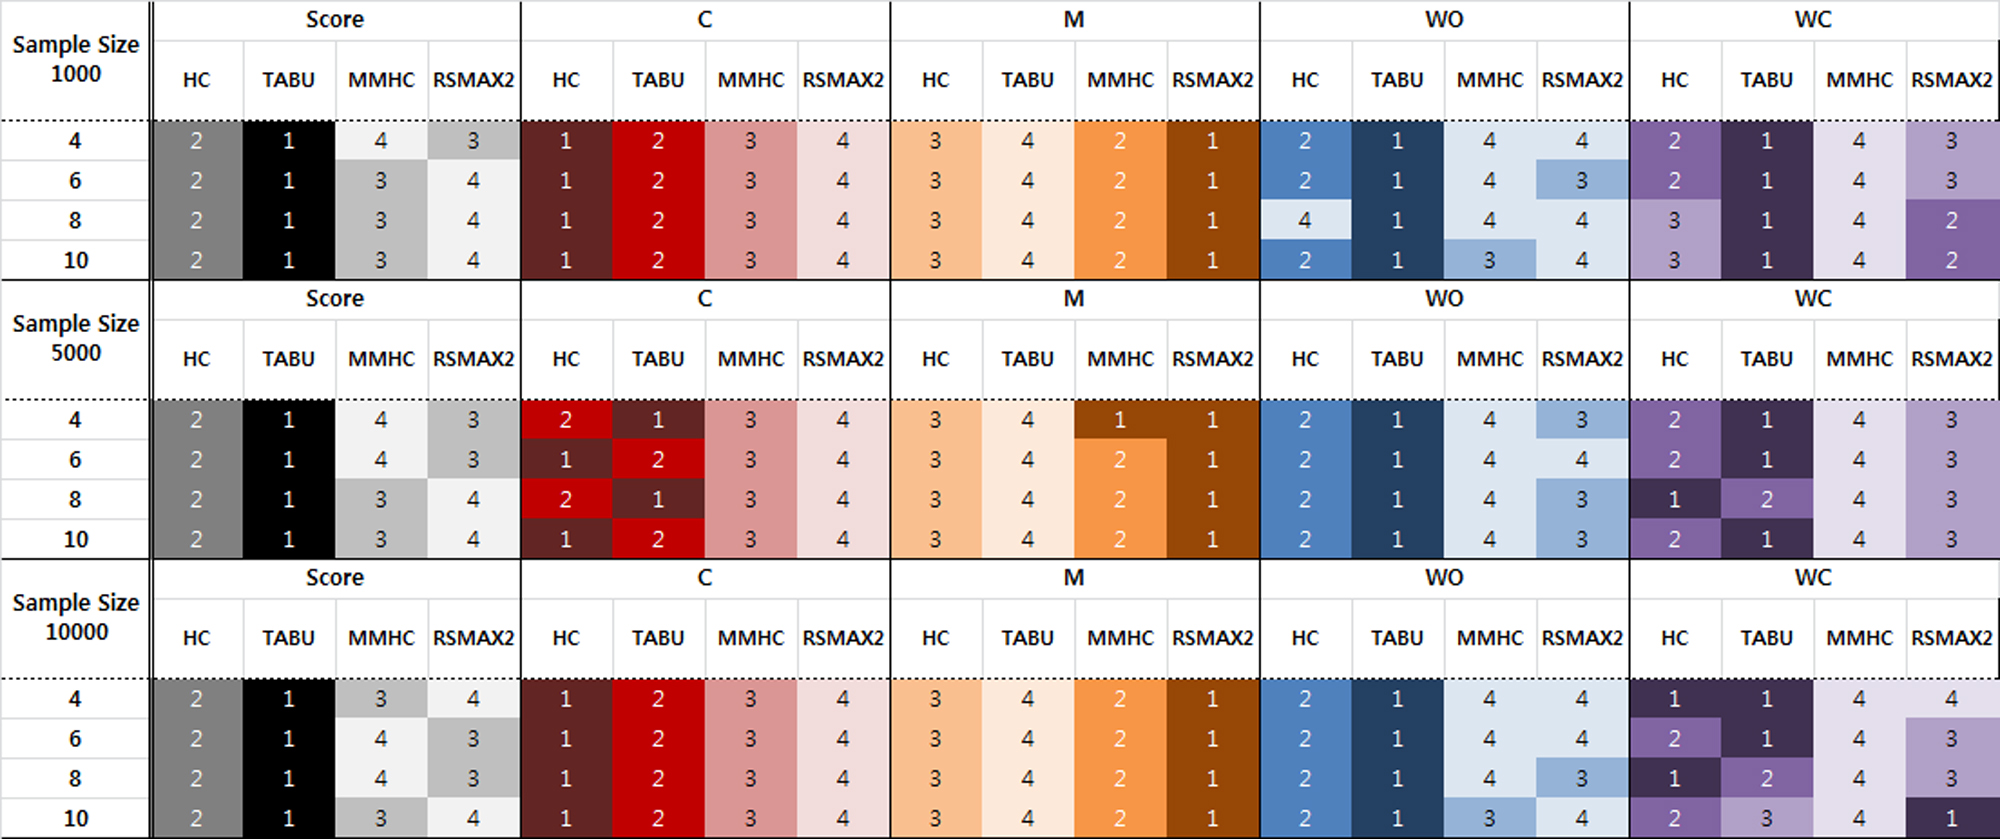
\includegraphics[height=170pt]{Result_Diamond}
		\caption{Summary for Comparison via Diamond}
	\end{figure}	

% Score, C 기준으로 비교했을 때 각각 TABU search, Hill-climbing이 좋은 성능을 나타냈다.
Score, respectively, when compared to the C standard TABU search, Hill-climbing showed a good performance.

% 하지만 WO, WC도 많은 것으로 나타났다.
However, WO, WC also showed that many.

% WO, WC가 적은 것을 기준으로 보았을 때 MMHC가 유리한 것으로 나타났다. RSMAX는 WC가 많이 나타났다.
WO, when WC is viewed by MMHC showed that less favorable. RSMAX showed a lot of WC.

% 이러한 현상은 sample size가 커질수록, node 개수가 많아질수록 두드러졌다.
This phenomenon is the larger the sample size, the greater the node count stood out.
	
	\begin{figure}[p]
	\centering
		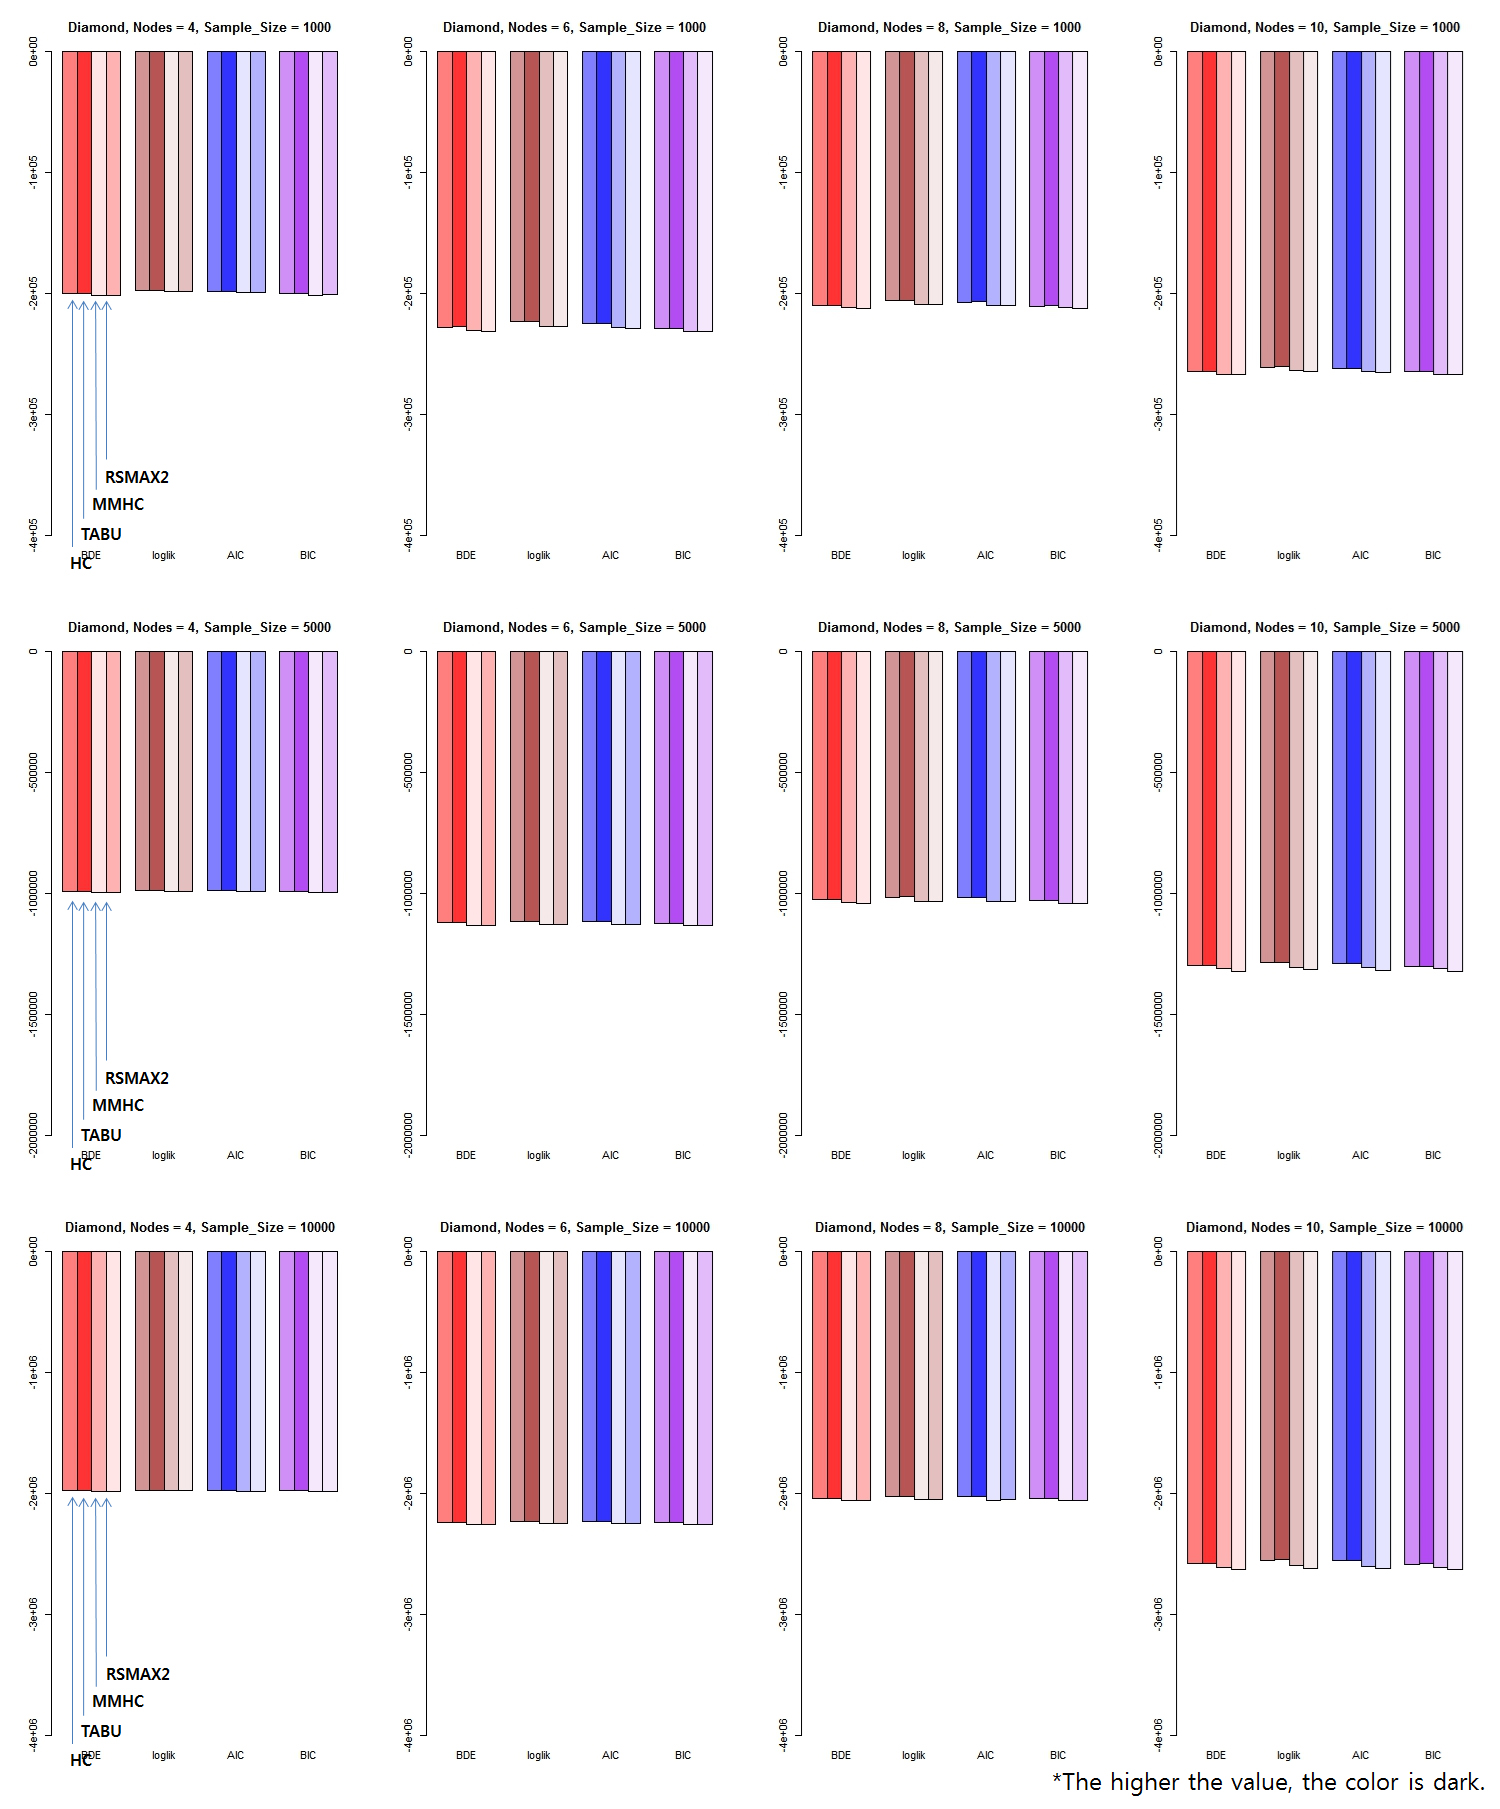
\includegraphics[height=500pt]{05_Diamond_Score}
		\caption{Comparison of scores via Diamond}
	\end{figure}	

	\begin{figure}[p]
	\centering
		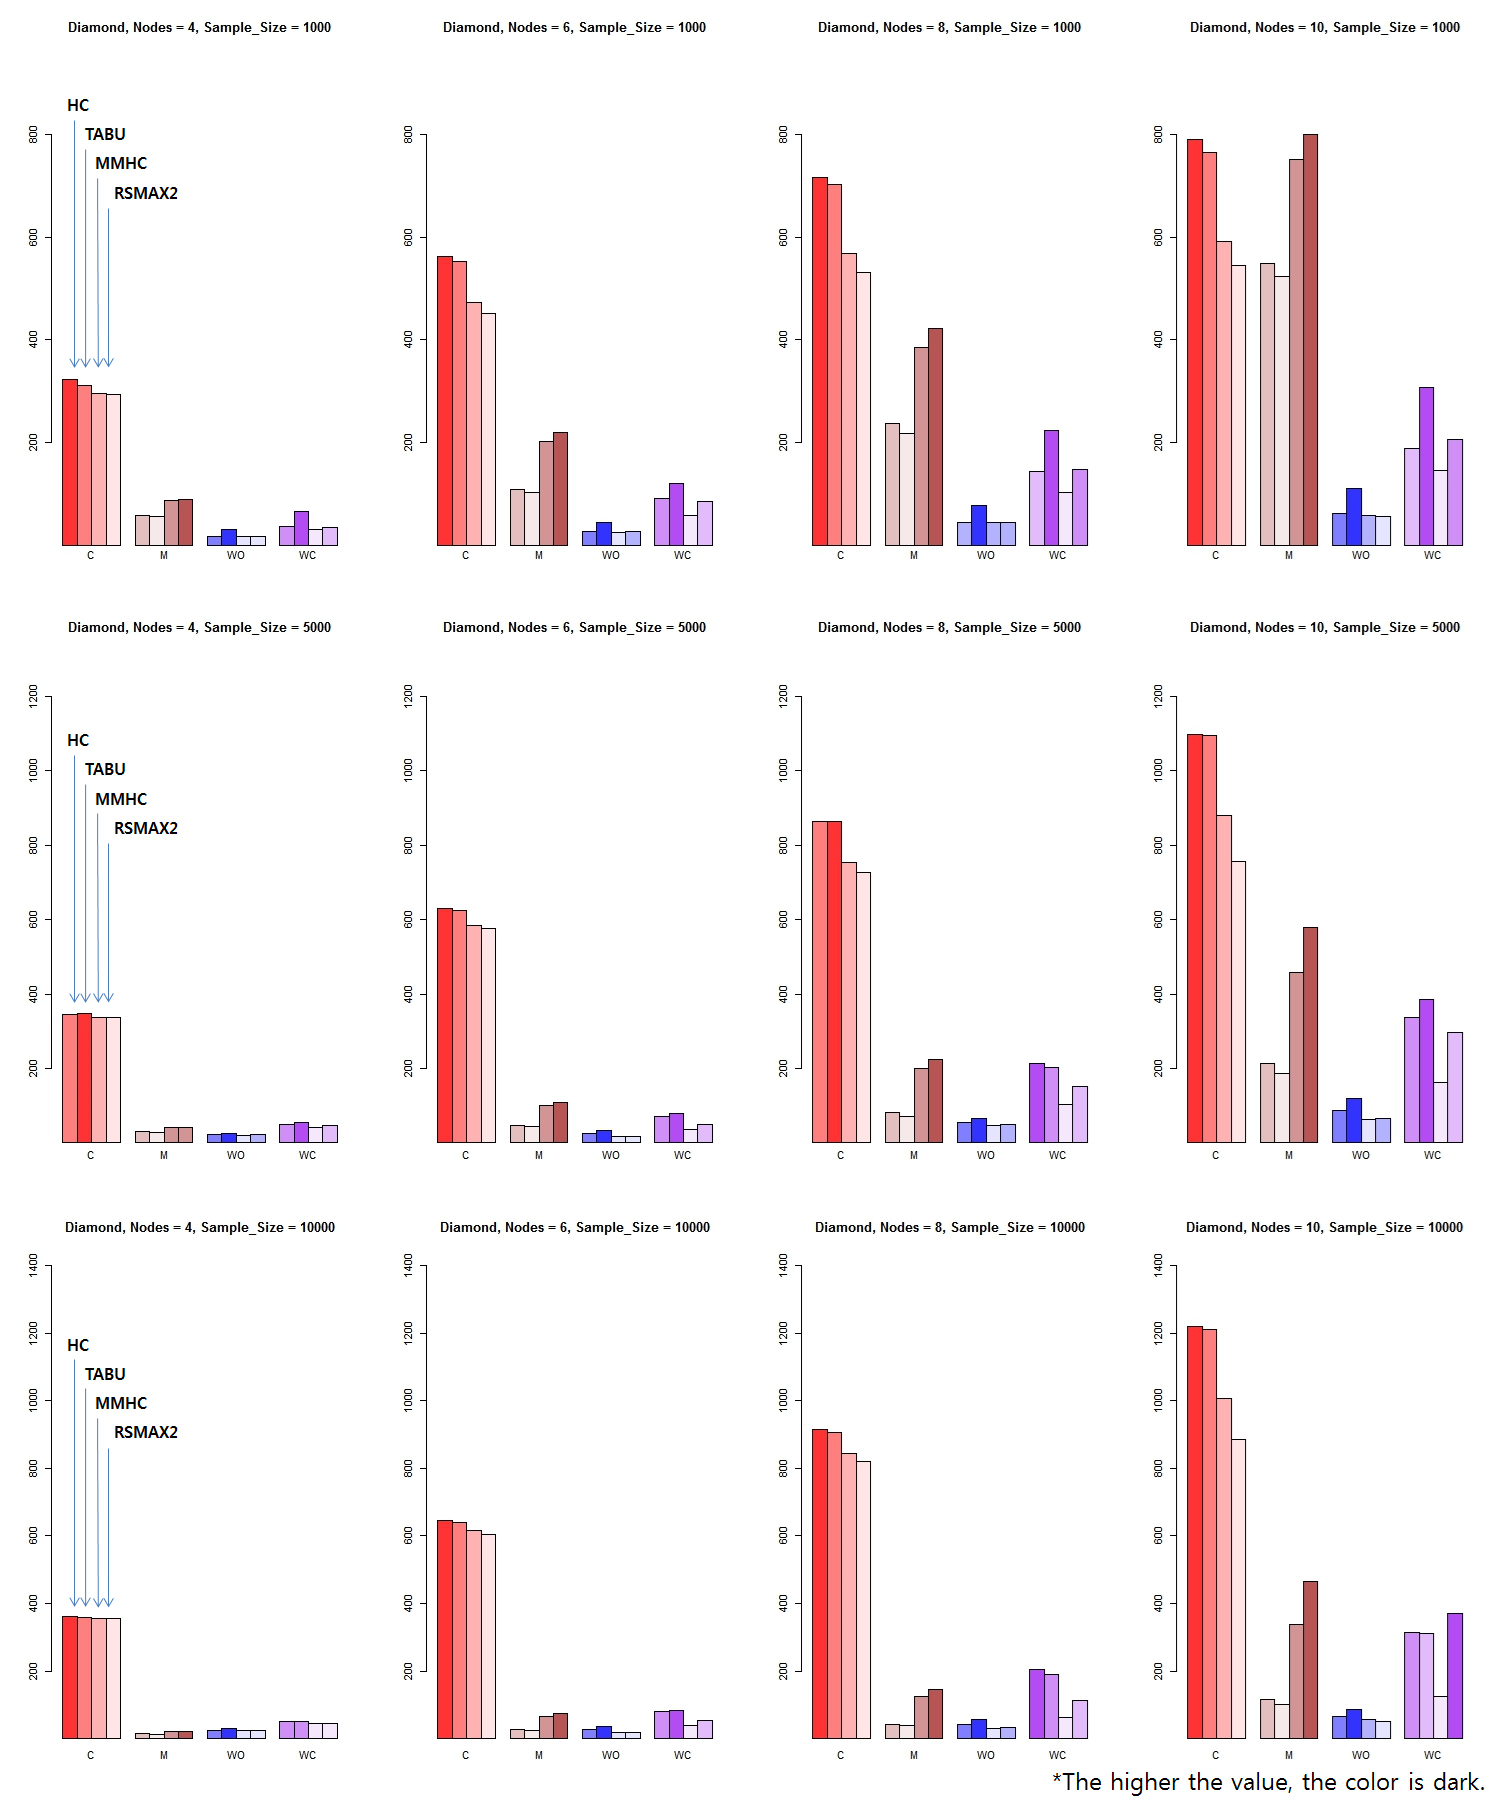
\includegraphics[height=500pt]{05_Diamond_Arcs}
		\caption{Comparison of correct arcs via Diamond}
	\end{figure}	
	